\documentclass{article}
\usepackage[pdftex]{hyperref}
\usepackage{float}
\usepackage{graphicx}

\begin{document}
\section{User-space Paging}

Fast memory paging is essential for general-purpose ``emerging applications'' such as those on smartphones, where cases like app startup rely on fast fault handling to reduce startup latency for the user.
\citet{Chen_JWLLLWHLYWYPX_24} claim that microkernels are inherently disadvantaged when servicing a page fault.
On a microkernel, the fault must be redirected to the memory pager server, which uses a kernel invocation to map the page to a memory frame, using a capability to the frame to do so.
In contrast, on a monolithic kernel, the fault can be directly serviced by the kernel.
\citet{Chen_JWLLLWHLYWYPX_24} make the claim that a ``significant performance degradation [...] due to the slow paging procedure of anonymous memory'' is observed, that is ``primarily due to the extra round-trip from the kernel to the pager''.
A secondary claim is that ``capabilities [...] introduce significant performance overhead due to the frequent updating of some kernel objects (e.g., the page table) managed outside the kernel and inhibit efficient cooperation between them [...] causing the handling of anonymous page faults 3.4$\times$ slower than Linux''.

Due to this, the pager has been moved inside the kernel in HongMeng, eliminating the extra round-trip IPC. The kernel pager, on a fault, directly maps a pre-allocated memory frame to the faulting page and then records an operations log for the user-space memory manager server to implement policies \citep{Chen_JWLLLWHLYWYPX_24}.
This departs from Liedtke's minimality principle \citep{Liedtke_95}, and we believe that their justification for this design choice is not sufficiently substantiated.

\subsection{HongMeng benchmarks}
\begin{figure}[H]
    \centering
    \resizebox{\textwidth}{!}{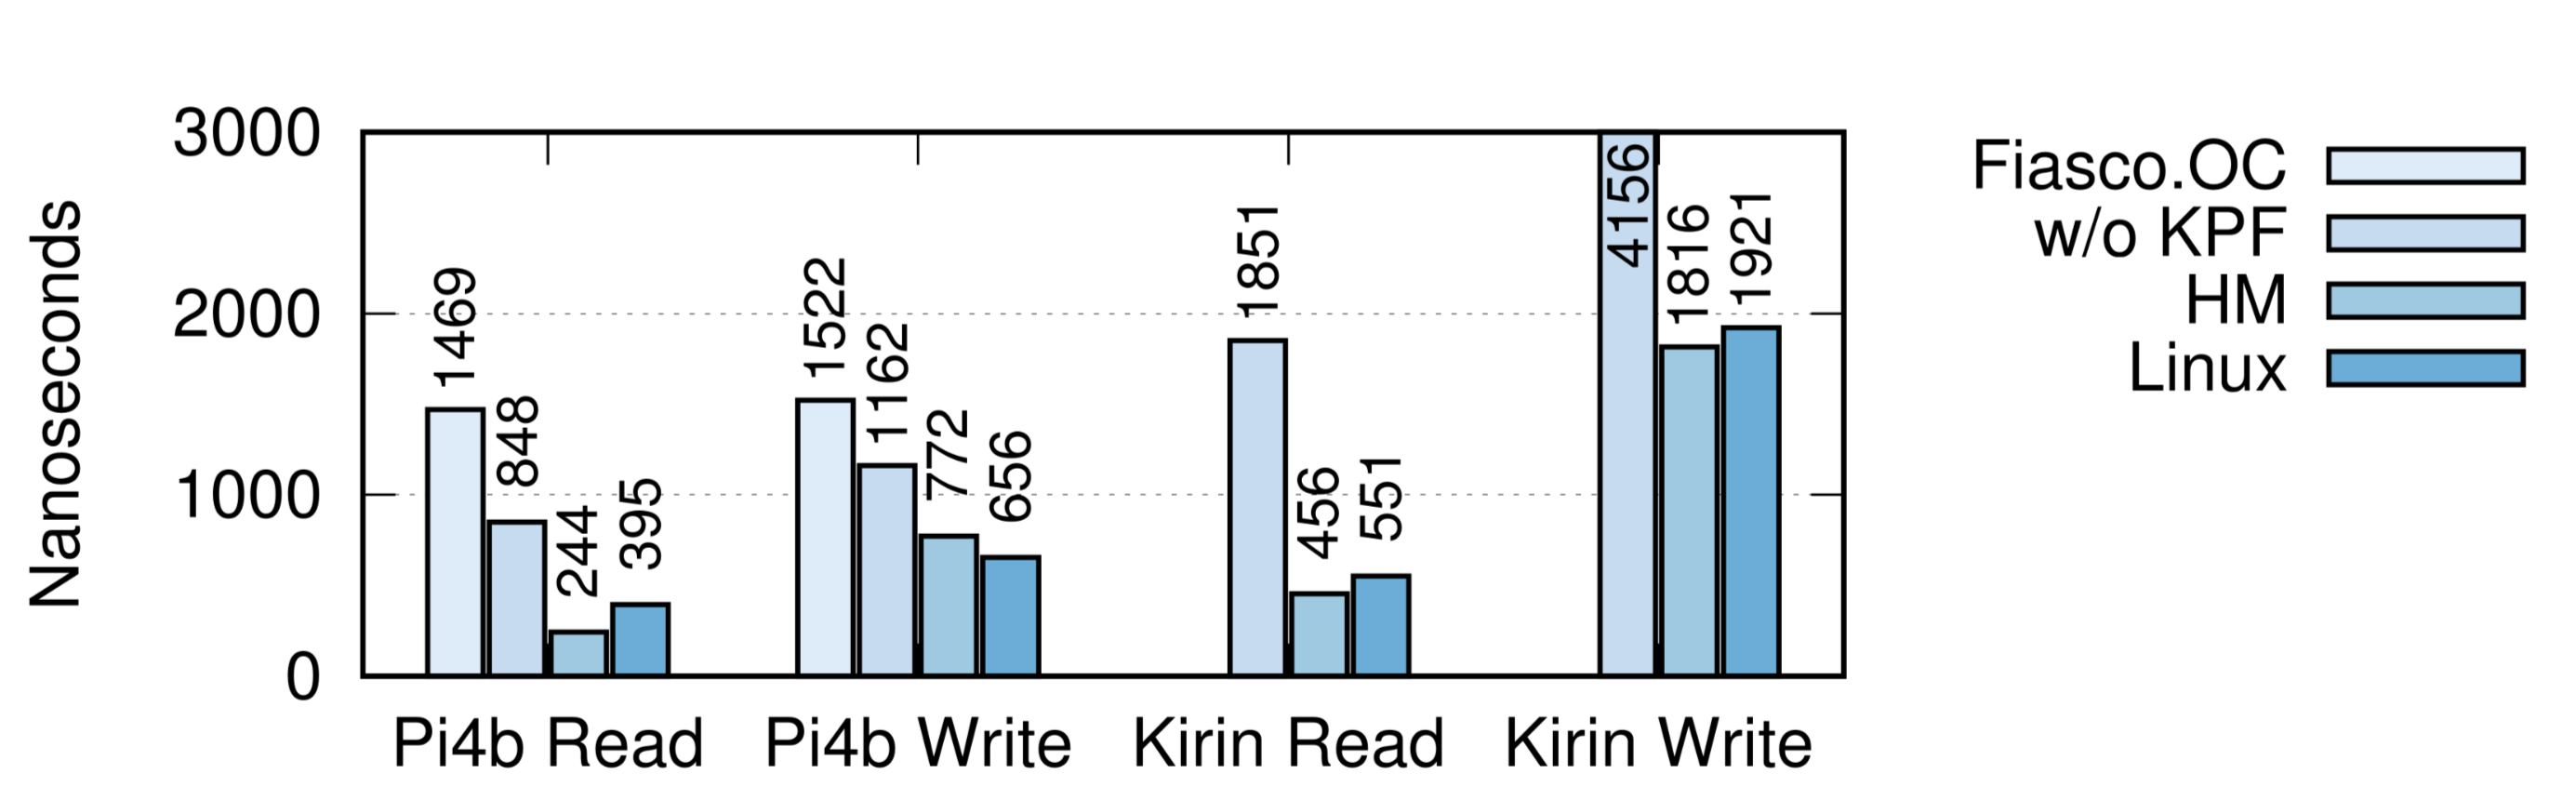
\includegraphics{mpfl-hm.png}}
    \caption{Page fault latency of private anonymous memory: HongMeng.}
    \label{mpfl-hm}
    w/o KPF denotes the HongMeng kernel with a user-space pager.\\
    This benchmark involved mapping anonymous memory via \textit{mmap} without pre-populating, then performing page-by-page operations to trigger page faults on first access. The benchmark measured average latency, calculated by triggering a batch of page faults and measuring the total elapsed time, and dividing it by the number of pages.
    Source: \citep{Chen_JWLLLWHLYWYPX_24}
\end{figure}

\autoref{mpfl-hm} shows the performance improvement of page fault latency that \citet{Chen_JWLLLWHLYWYPX_24} achieved in the HongMeng kernel by moving the pager into the kernel.
On the Pi4b, they record a latency reduction of 72\%/33\% on Pi4b and 75\%/55\% on Kirin9000 (little core). The Linux versions used for comparison here are 6.1 for Pi4b and 5.10 for Kirin.

\subsection{Argument for user-space paging}
The argument is that the IPC cost and frame capability invocation (from mapping) are not as significant a cause of performance degradation as claimed by \citet{Chen_JWLLLWHLYWYPX_24}.
It should be possible to implement performant (similar to Linux) user-space paging without compromising on a principled microkernel design.
Thus, a user-space pager on LionsOS (which is based on seL4) should demonstrate that private anonymous page fault latency similar to that of Linux can be achieved on a traditional (unmodified) microkernel.
We do this by replicating the private anonymous page fault latency experiment of \citet{Chen_JWLLLWHLYWYPX_24}, depicted in Figure 8 of ``Microkernel Goes General: Performance and Compatibility in the HongMeng Production Microkernel.''

\subsection{Our benchmarking}
% results shown..
\begin{figure}[H]
    \centering
    \resizebox{\textwidth}{!}{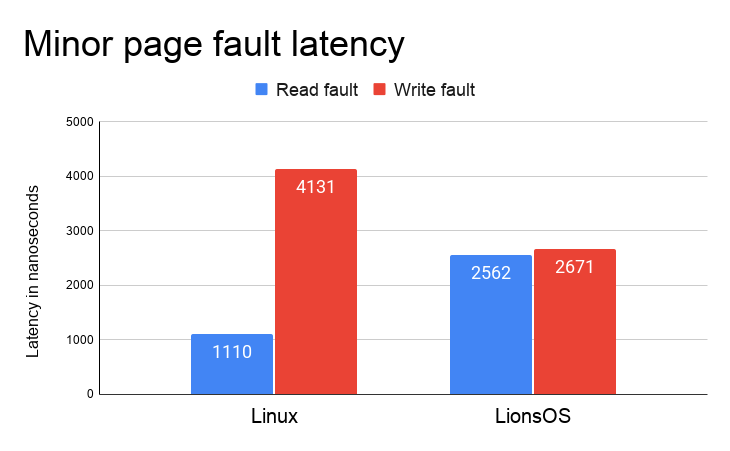
\includegraphics{mpfl.png}}
    \caption{Page fault latency of private anonymous memory: LionsOS.}
    \label{lionsos-mpfl}
    Measured on Pi4b with a 1.5GHz clock rate. Linux version is 6.12.61-v8. Read is optimised with zero page.

\end{figure}
\autoref{lionsos-mpfl} shows our benchmarking of page fault latency which follows the same methodology as in \autoref{mpfl-hm}.
This benchmark shows the average page fault latency measured by triggering a batch of page faults and measuring the total elapsed time divided by the number of pages. This was run for 16384 4096 byte pages on Pi4b running at 1.5GHz clock frequency.
The page faults were triggered by accessing private anonymous, not pre-populated memory, mapped via \textit{mmap}.

% Explain what my pager does while servicing the benchmark
\textbf{Write fault}\\
The general process to service write faults is: \begin{enumerate}
    \item Get a (pre-allocated) frame cap to an unused memory frame.
    \item Create shadow page tables to keep track of this frame.
    \item Map (pre-allocated) intermediary paging structures.
    \item Map frame cap to faulting page.
    \item Resume execution on faulting PD
\end{enumerate}

\textbf{Read fault}\\
The \texttt{mmap()} syscall allocates zero-filled pages, hence the global zero-page optimisation is triggered for Linux, requiring less bookkeeping as the global zero page can simply be read-only mapped.
The LionsOS pager also implements the same optimisation, mapping a global zero frame.
However, as the same frame cannot be mapped into the same vspace using the same capability, a pre-allocated capability copy must be used to do the mapping, and as we cannot lose track of the capability (as we do not want to leak CNode slots), we must also create shadow page tables for this capability copy and map this frame to the faulting page.
This results in a similar amount of bookkeeping as write faults and the same number of kernel invocations (mapping intermediary paging structures and page mapping) resulting in a similar latency.
\autoref{mpfl-hm} shows that this affects Fiasco.OC similarly as they also use a similar capability model and therefore read and write fault latencies are not significantly different.

\autoref{lionsos-mpfl} shows an approximate average latency of 2600ns per fault for both write and read faults. The \texttt{PAGE\_MAP} operation accounts for approximately 847-885ns (read, write). Approximately 200-300ns are used for bookkeeping and the rest is accounted for by the fault delivery and round trip IPC. The pager is implemented as a passive server to reduce scheduling overhead.

% conclusion.
\subsection{Conclusion}
We observe from \autoref{lionsos-mpfl} that write fault handling can be done with a lower latency than Linux, despite the inclusion of the extra round-trip IPC and capability operations. The global zero-page optimisation is approximately 2.5$\times$ slower than Linux, but this is an edge case optimisation that only occurs on reads to zeroed out pages or previously unaccessed pages. The slowdown cited by \citet{Chen_JWLLLWHLYWYPX_24} is not as significant for the read case and for the write case, LionsOS achieves better performance, contradicting their claims.

This shows that the argument for introducing the pager into the kernel to achieve better performance is not so obvious. In order to keep the option of functional verification for the kernel open, the pager should be implemented as a user-space server.

\subsection{Weird results from \autoref{mpfl-hm}}
I failed to match the measurements from \citet{Chen_JWLLLWHLYWYPX_24}, and here are some weird things I have noticed that confuse me:
\begin{itemize}
    \item Kirin 9000 (little core) which is a cortex a55 at 2.05GHz is drastically slower than Pi4b which is a cortex a73 at 1.5GHz.
    \item Fiasco.OC achieves around 1500ns latency per fault. This is 2250 cycles to do the IPC and fault delivery, mapping operations and bookkeeping. Given that their fastpath IPC is slower than seL4's, this seems implausible.
    \item \citet{Chen_JWLLLWHLYWYPX_24} claims for seL4 that ``the round-trip (to the pager) of fault handling takes about 140ns on Pi4b (measured using sel4bench), which makes it significantly slower than Linux.'' This is a strange claim to me as a round-trip IPC fastpath on seL4 on Armv8a takes around 1000 cycles, not the 210 cycles claimed here.
\end{itemize}
\bibliographystyle{plainnat}
\bibliography{references}
\end{document}